\documentclass[12pt]{article}

\usepackage{pdfpages}
\usepackage{graphicx}
\usepackage{float}

\title{Project Progress Update}
\author{Ian Ooi}
\date{Due April 15, 2014}

\begin{document}
	\maketitle
	\section{Storyboard}
		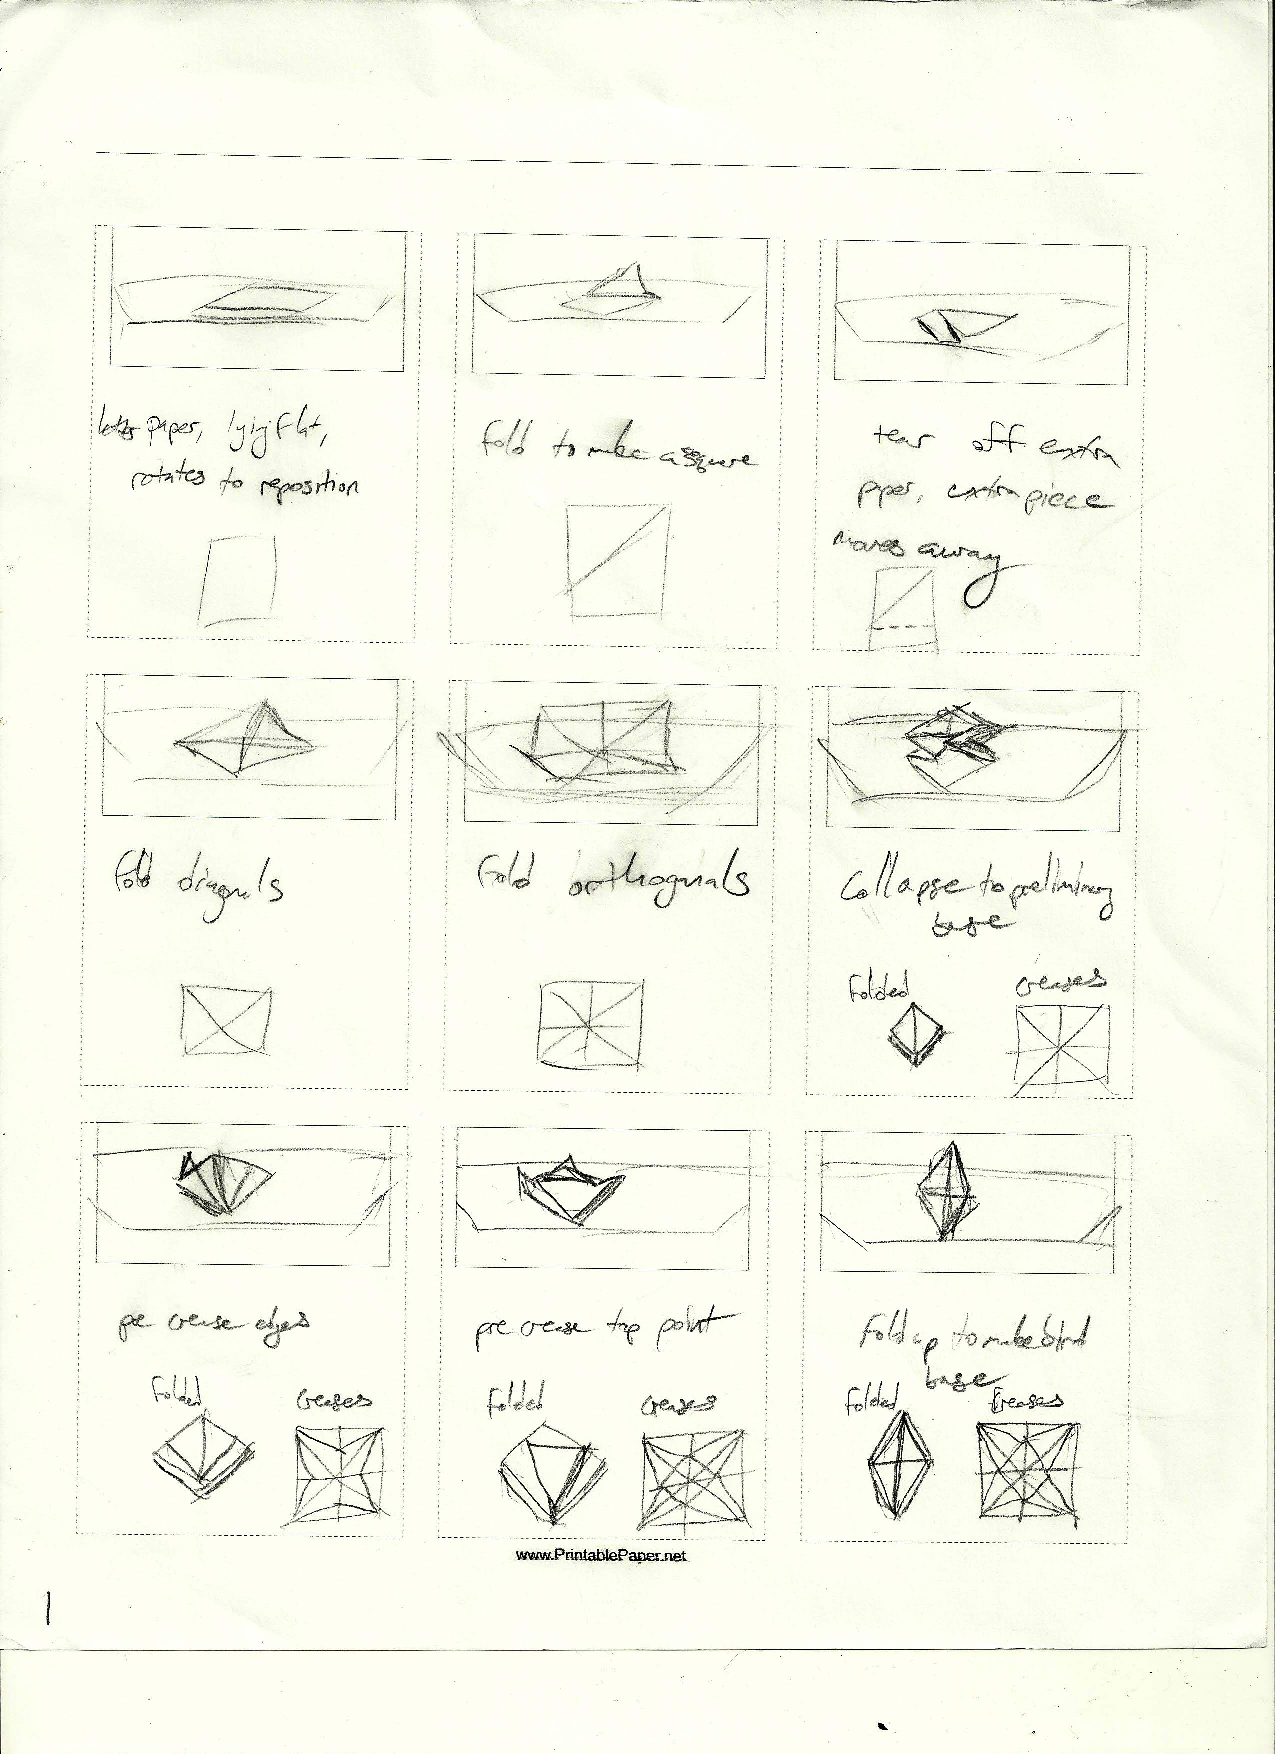
\includepdf[pages={1,2,3}]{storyboard.pdf}
	\section{Related Work}
		Stop motion is a style chosen for its aesthetics and production style.  Films such as Coraline, Paranorman, Wallace and Gromit, Chicken Run, the Corpse Bride, and the shorts by PES such as Fresh Guacamole.  Low cost and improved detail and texture are both factors in the choice to use stop motion, in addition to the distinctive style.  The relative ease of production, subject matter (origami is fairly conducive to stop motion as it is static, positionable, and somewhat rigid in its movements), and cleanliness of the frames (i.e. no motion blur or similar effects) contributed to the choice of stop motion.
		
		Inpainting and compositing are commonly used effects in the field of visual effects, and can be used in conjunction with stop motion to remove any wires, stands, and pieces that are used for structure, support and positioning but are not intended for the final cut.  The techniques are described in Computer Vision for Visual Effects by Radke.
		
	\section{Data Collection}
		Data was collected in mostly one burst.  A Canon camera was set up on a tripod overlooking the scene, which was then posed and photographed to produce the next frame.  The camera was fitted with a 50mm prime lens, and was set with 1/30 shutter speed, f-stop of 13, and ISO 2000.  A dark blue background was used for the folding shots as well as for the flapping wing sequence.  Outdoor scenes are to be collected on the next clear (or somewhat clear) day to attempt to get blue skies.
		
	\section{Technical Approach}
		The frames are captured with minimal supports for the model.  Wires are used for propping up and manipulating the model frame to frame, ensuring controlled maneuvers.  A static tripod setup was used to ensure consistency between frames.	
		
		From this setup, it is a simple matter of using image compositing and inpainting to remove wires and stands from the frames.  Some frames were harder to set up, and were captured with manual positioning of the crane (i.e. I was holding it with my hand).  Patchmatch implementations are available in tools such as photoshop, and code implementations can be found for inpainting techniques on the internet.  Image compositing and matting samples can also be found.  The wires used were generally green in color to differentiate from the background used, so a simple detection scheme could be used to find the wires and remove them in a batch edit as opposed to editing each frame.  This would be the final goal.  A tracking system could also be used, but due to the nature of the footage, it shouldn't be required.  For the outdoor sequence, the images should be composited onto the backgrounds, again as a batch.
		
	\section{Sample Frames}
		\begin{figure}[H]
			\centering
			\includegraphics[width=0.3\textwidth]{frame_samples/IMG_3056.JPG}
			\includegraphics[width=0.3\textwidth]{frame_samples/IMG_3057.JPG}
			\includegraphics[width=0.3\textwidth]{frame_samples/IMG_3058.JPG}
			\includegraphics[width=0.3\textwidth]{frame_samples/IMG_3059.JPG}
			\includegraphics[width=0.3\textwidth]{frame_samples/IMG_3060.JPG}
		\end{figure}
	\section{Plan for Completion and Further Work}
		I have yet to capture outside shots for the final part of the sequence where the crane flies outside.  Currently, the results I have are based off of image compositing, but for some inpainting would likely produce better results.  I need to test this, and then go through with the inpainting approach where necessary.  The matting seems to work reasonably, but I will need to inspect the actual appearance of the bird when composited onto the outdoor scene.  Lighting especially concerns me, where the lighting on the bird may be inconsistent with the outdoor scene.
\end{document}